\documentclass[12pt,letterpaper]{article}
\usepackage{graphicx,textcomp}
\usepackage{natbib}
\usepackage{setspace}
\usepackage{fullpage}
\usepackage{color}
\usepackage[reqno]{amsmath}
\usepackage{amsthm}
\usepackage{fancyvrb}
\usepackage{amssymb,enumerate}
\usepackage[all]{xy}
\usepackage{endnotes}
\usepackage{lscape}
\newtheorem{com}{Comment}
\usepackage{float}
\usepackage{hyperref}
\newtheorem{lem} {Lemma}
\newtheorem{prop}{Proposition}
\newtheorem{thm}{Theorem}
\newtheorem{defn}{Definition}
\newtheorem{cor}{Corollary}
\newtheorem{obs}{Observation}
\usepackage[compact]{titlesec}
\usepackage{dcolumn}
\usepackage{tikz}
\usetikzlibrary{arrows}
\usepackage{multirow}
\usepackage{xcolor}
\newcolumntype{.}{D{.}{.}{-1}}
\newcolumntype{d}[1]{D{.}{.}{#1}}
\definecolor{light-gray}{gray}{0.65}
\usepackage{url}
\usepackage{listings}
\usepackage{color}

\definecolor{codegreen}{rgb}{0,0.6,0}
\definecolor{codegray}{rgb}{0.5,0.5,0.5}
\definecolor{codepurple}{rgb}{0.58,0,0.82}
\definecolor{backcolour}{rgb}{0.95,0.95,0.92}

\lstdefinestyle{mystyle}{
	backgroundcolor=\color{backcolour},   
	commentstyle=\color{codegreen},
	keywordstyle=\color{magenta},
	numberstyle=\tiny\color{codegray},
	stringstyle=\color{codepurple},
	basicstyle=\footnotesize,
	breakatwhitespace=false,         
	breaklines=true,                 
	captionpos=b,                    
	keepspaces=true,                 
	numbers=left,                    
	numbersep=5pt,                  
	showspaces=false,                
	showstringspaces=false,
	showtabs=false,                  
	tabsize=2
}
\lstset{style=mystyle}
\newcommand{\Sref}[1]{Section~\ref{#1}}
\newtheorem{hyp}{Hypothesis}


\title{Problem Set 4}
\date{Due: December 3, 2023}
\author{Applied Stats/Quant Methods 1}


\begin{document}
	\maketitle
	\section*{Instructions}
	\begin{itemize}
		\item Please show your work! You may lose points by simply writing in the answer. If the problem requires you to execute commands in \texttt{R}, please include the code you used to get your answers. Please also include the \texttt{.R} file that contains your code. If you are not sure if work needs to be shown for a particular problem, please ask.
		\item Your homework should be submitted electronically on GitHub.
		\item This problem set is due before 23:59 on Sunday December 3, 2023. No late assignments will be accepted.
	\end{itemize}



	\vspace{.5cm}
\section*{Question 1: Economics}
\vspace{.25cm}
\noindent 	
In this question, use the \texttt{prestige} dataset in the \texttt{car} library. First, run the following commands:

\begin{verbatim}
install.packages(car)
library(car)
data(Prestige)
help(Prestige)
\end{verbatim} 


\noindent We would like to study whether individuals with higher levels of income have more prestigious jobs. Moreover, we would like to study whether professionals have more prestigious jobs than blue and white collar workers.

\newpage
\begin{enumerate}
	
	\item [(a)]
	Create a new variable \texttt{professional} by recoding the variable \texttt{type} so that professionals are coded as $1$, and blue and white collar workers are coded as $0$ (Hint: \texttt{ifelse}).
	
	\noindent First, I thoroughly review the data set in addition to what is suggested:
	
	\lstinputlisting[language=R, firstline=47, lastline=53]{PS4.R}  
	
	\noindent Next, I check the levels of \texttt{type} to inform the ifelse expression for creating a new variable \texttt{professional}
	
	\lstinputlisting[language=R, firstline=58, lastline=59]{PS4.R}

	\noindent Lastly, I create a new dummy variable \texttt{professional}, and then coerce it as a factor to ensure the following model does not interpret the variable as a continuous numerical variable.

	\lstinputlisting[language=R, firstline=61, lastline=68]{PS4.R}
	
	\item [(b)]
	Run a linear model with \texttt{prestige} as an outcome and \texttt{income}, \texttt{professional}, and the interaction of the two as predictors (Note: this is a continuous $\times$ dummy interaction.)
	
	\noindent I run the linear model. Note that the \texttt{lm()} function omits observations which include at least one NA value among selected variables by default. In this case, I specify.

	\lstinputlisting[language=R, firstline=74, lastline=74]{PS4.R}
	
		\begin{table}[!h]
			\centering 
			\caption{Model 1 Regression Table} 
			\label{} 
			\begin{tabular}{@{\extracolsep{5pt}}lD{.}{.}{-3} } 
				\\[-1.8ex]\hline 
				\hline \\[-1.8ex] 
				& \multicolumn{1}{c}{\textit{Dependent variable:}} \\ 
				\cline{2-2} 
				\\[-1.8ex] & \multicolumn{1}{c}{Prestige Score} \\ 
				\hline \\[-1.8ex] 
				Income (\$1) & 0.003^{***} \\ 
				& (0.0005) \\ 
				& \\ 
				Professional = 1 & 37.781^{***} \\ 
				& (4.248) \\ 
				& \\ 
				Interaction term: Income and Professional = 1 & -0.002^{***} \\ 
				& (0.001) \\ 
				& \\ 
				Constant & 21.142^{***} \\ 
				& (2.804) \\ 
				& \\ 
				\hline \\[-1.8ex] 
				Observations & \multicolumn{1}{c}{98} \\ 
				R$^{2}$ & \multicolumn{1}{c}{0.787} \\ 
				Adjusted R$^{2}$ & \multicolumn{1}{c}{0.780} \\ 
				Residual Std. Error & \multicolumn{1}{c}{8.012 (df = 94)} \\ 
				F Statistic & \multicolumn{1}{c}{115.878$^{***}$ (df = 3; 94)} \\ 
				\hline 
				\hline \\[-1.8ex] 
				\textit{Note:}  & \multicolumn{1}{r}{$^{*}$p$<$0.1; $^{**}$p$<$0.05; $^{***}$p$<$0.01} \\ 
			\end{tabular} 
		\end{table} 

	\noindent Interpretations for \textbf{Income} and \textbf{Professional = 1} are discussed in following questions. I note the Interaction term represents the average diminished effect of Income on Prestige Score for Professional workers. In other words, the average effect of increasing income by \$1 on a worker's Prestige Score is, on average, less for professional workers than for white/blue-collar workers (see Figure 1).
	
	\begin{figure}[!h]
		\centering
		\caption{Marginal Effect of Income on Prestige}
		\label{}
		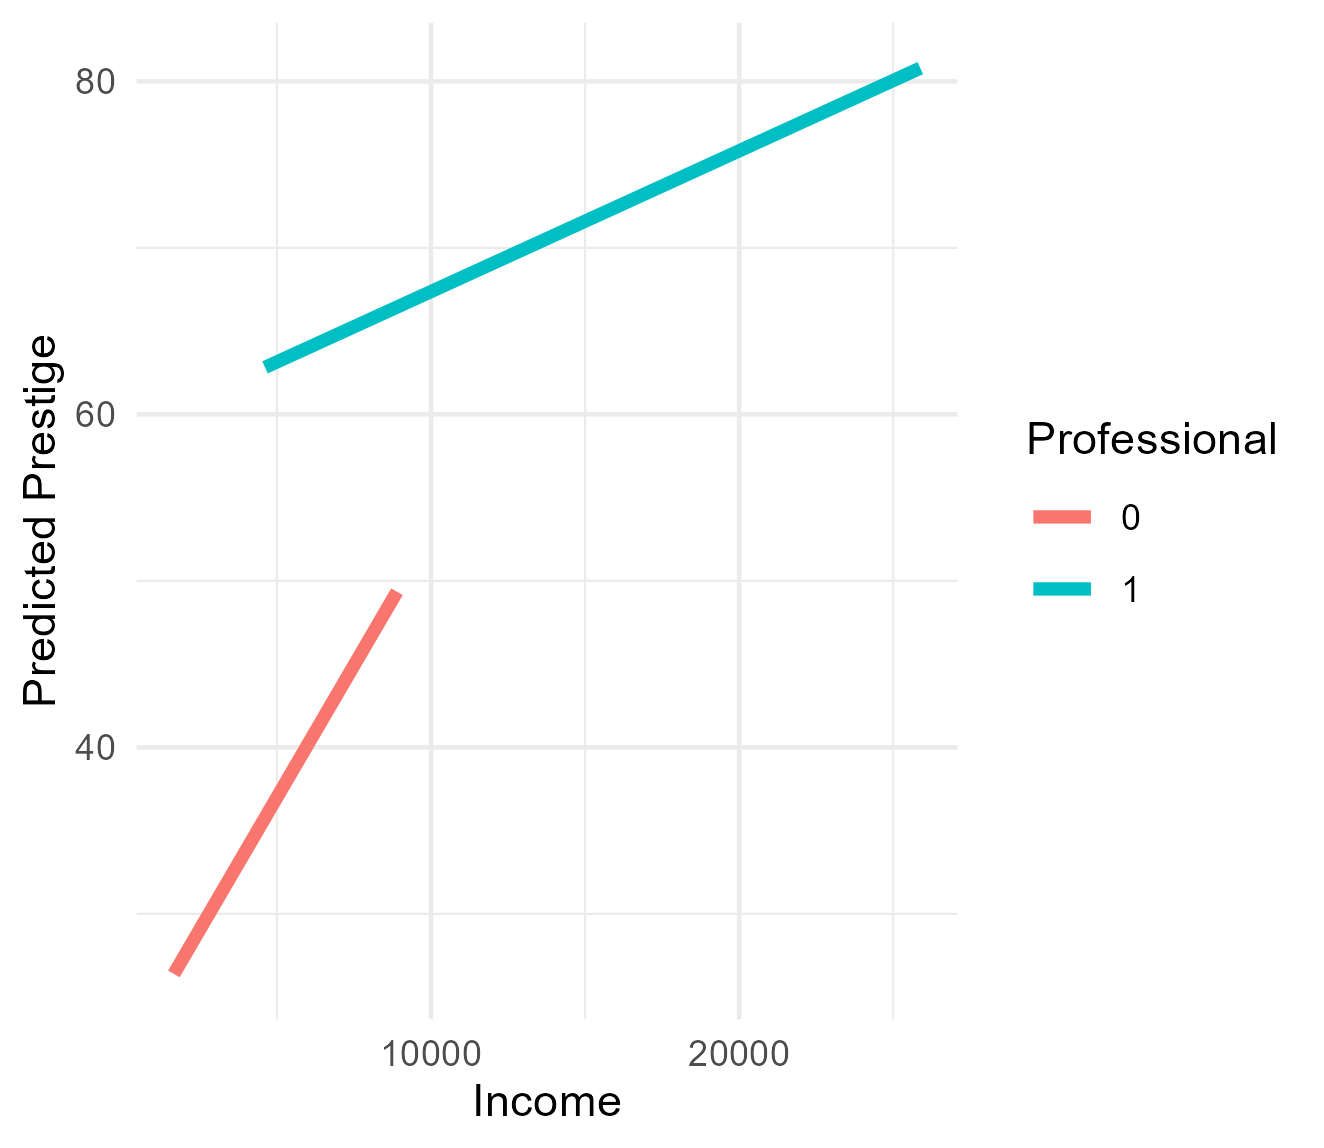
\includegraphics[width=0.8\textwidth]{marginal_effect_plot.png}
	\end{figure}
	
	The Constant term represents the average Prestige Score for a white/blue-collar worker with \$0 income (or the lowest possible value in Income).
	
	$R^2$ indicates the model predicts 78.7\% of the variation in observed \texttt{Prestige Score} in the data set.
	\texttt{F Statistic} represents the hypothesis test that at least one of the partial effects (the coefficients) in the model is non-zero. In this case, the F-value is less than 0.05 and so gives evidence to reject the null hypothesis that all partial effects are equal to zero, and gives evidence for the alternative hypothesis that at least one of the partial effects is non-zero.
	
	\newpage
	\item [(c)]
	Write the prediction equation based on the result.
	
	\noindent The following is a generic equation with two predictor variables $X$ and $D$, an interaction term between the two, and stochastic error.
	
	Note the stochastic error is assumed to cancel out given the assumptions for linear regression: $\varepsilon_i \stackrel{iid}{\sim} N(O, \sigma^2)$ (independence, normality, and constant variance of errors).
	
	\begin{align*}
		Y_i &= \beta_0 + \beta_1 X_i + \beta_2 D_i + \beta_3 X_i D_i + \varepsilon_i
	\end{align*}

	\noindent Below I input the prediction equation values:
	
	\begin{align*}
		\text{prestige} = 21.142 + 0.003 \times  \text{income} + 37.781 \times  \text{professional} + (-0.002 \times  \text{income} \times \text{professional)}
	\end{align*}
	
\newpage
	\item [(d)]
	Interpret the coefficient for \texttt{income}.
	
	\noindent The coefficient for \textbf{income} represents the average increase in prestige per one additional dollar of income for white- and blue-collar workers (a.k.a. holding the professional variable constant).
	
	Further, the p-value for the coefficient is less than the typcial $\alpha = 0.05$, therefore giving evidence to reject the null hypothesis that the partial effect of income on prestige for white/blue-collar workers is zero, and giving evidence for the alternative hypothesis that the partial effect of income on prestige for white/blue-collar workers is non-zero.
	
	\item [(e)]
	Interpret the coefficient for \texttt{professional}.
	
	\noindent The coefficient for \textbf{professional} represents the average increase in prestige for an individual who moves from white-/blue-collar employment to 'professional' employment, holding income constant.
	
	Further, the p-value for the coefficient is less than the typcial $\alpha = 0.05$, therefore giving evidence to reject the null hypothesis that the partial effect of moving from white/blue-collar to professional employment is zero, holding income constant, and giving evidence for the alternative hypothesis that the partial effect is non-zero, holding income constant.
	
	\item [(f)]
	What is the effect of a \$1,000 increase in income on prestige score for professional occupations? In other words, we are interested in the marginal effect of income when the variable \texttt{professional} takes the value of $1$. Calculate the change in $\hat{y}$ associated with a \$1,000 increase in income based on your answer for (c).
	
	\noindent I am comparing the average increase in estimated prestige for a professional when their income increases from \$0 to \$1000.
	
	\begin{align*}
		\text{prestige}_{professional + \$0} &= 21.142 + 0.003 \times  0 + 37.781 \times  1 + (-0.002 \times  0 \times 1)\\
		&= 21.142 + 37.781 \times  1\\
		&= 58.92\\
		\text{prestige}_{professional + \$1000} &= 21.142 + 0.003 \times  1000 + 37.781 \times  1 + (-0.002 \times  1000 \times 1)\\
		&= 59.77
	\end{align*}
	
	\lstinputlisting[language=R, firstline=110, lastline=114]{PS4.R}
	
	\noindent Subtracting the estimated prestige score of a professional with \$0 from that of a professional with \$1000 indicates the (average) marginal effect of increasing an average professional's income from \$0 to \$1000 is an increase of 0.85 prestige-score points.

	\lstinputlisting[language=R, firstline=116, lastline=118]{PS4.R}
	
	\item [(g)]
	What is the effect of changing one's occupations from non-professional to professional when her income is \$6,000? We are interested in the marginal effect of professional jobs when the variable \texttt{income} takes the value of $6,000$. Calculate the change in $\hat{y}$ based on your answer for (c).
	
	\begin{align*}
		\text{prestige}_{non-professional + \$6000} &= 21.142 + 0.003 \times  6000\\
		&= 40.17\\
		\text{prestige}_{professional + \$6000} &= 21.142 + 0.003 \times  6000 + 37.781 \times  1 + (-0.002 \times  6000 \times 1)\\
		&= 63.99\\
	\end{align*}	
	
	\lstinputlisting[language=R, firstline=122, lastline=126]{PS4.R}	
	
	\noindent Subtracting the estimated prestige score of a non-professional with \$6000 from that of a professional with \$6000 indicates the marginal (average) effect of moving from white/blue-collar employment to professional employment, when income is constant at \$6000, is associated with an average increase of 23.83 prestige-score points.
	
	\lstinputlisting[language=R, firstline=128, lastline=130]{PS4.R}	
	
\end{enumerate}

\newpage

\section*{Question 2: Political Science}
\vspace{.25cm}
\noindent 	Researchers are interested in learning the effect of all of those yard signs on voting preferences.\footnote{Donald P. Green, Jonathan	S. Krasno, Alexander Coppock, Benjamin D. Farrer,	Brandon Lenoir, Joshua N. Zingher. 2016. ``The effects of lawn signs on vote outcomes: Results from four randomized field experiments.'' Electoral Studies 41: 143-150. } Working with a campaign in Fairfax County, Virginia, 131 precincts were randomly divided into a treatment and control group. In 30 precincts, signs were posted around the precinct that read, ``For Sale: Terry McAuliffe. Don't Sellout Virgina on November 5.'' \\

Below is the result of a regression with two variables and a constant.  The dependent variable is the proportion of the vote that went to McAuliff's opponent Ken Cuccinelli. The first variable indicates whether a precinct was randomly assigned to have the sign against McAuliffe posted. The second variable indicates
a precinct that was adjacent to a precinct in the treatment group (since people in those precincts might be exposed to the signs).  \\

\vspace{.5cm}
\begin{table}[!htbp]
	\centering 
	\textbf{Impact of lawn signs on vote share}\\
	\begin{tabular}{@{\extracolsep{5pt}}lccc} 
		\\[-1.8ex] 
		\hline \\[-1.8ex]
		Precinct assigned lawn signs  (n=30)  & 0.042\\
		& (0.016) \\
		Precinct adjacent to lawn signs (n=76) & 0.042 \\
		&  (0.013) \\
		Constant  & 0.302\\
		& (0.011)
		\\
		\hline \\
	\end{tabular}\\
	\footnotesize{\textit{Notes:} $R^2$=0.094, N=131}
\end{table}

\vspace{.5cm}
\begin{enumerate}
	\item [(a)] Use the results from a linear regression to determine whether having these yard signs in a precinct affects vote share (e.g., conduct a hypothesis test with $\alpha = .05$).
	
	\noindent I will conduct a t-test for the following hypothesis tests as the sample sizes for each group vary - treatment groups (n=30 and n=76) and control group (n=25) - two of which are below or at the margin of the typical cut-off point of n=30 for Z-scores.
	
	\begin{align*}
		H_0: \hat \beta_1 = 0\\
		H_a: \hat \beta_1 \neq 0
	\end{align*}
	
	\noindent The test statistic is calculated by dividing the difference between the coefficient and null hypothesis by the standard error:

	\begin{align*}
		t = \frac{ \hat \beta - \beta_{H_0}}{\hat \sigma_{\hat \beta}}
	\end{align*}
	
	\texttt Below is the t-score for the coefficient representing the change in precinct voting preference correlated with assignment of lawn signs:
	
	\begin{align*}
		2.625 = \frac{0.042 - 0}{0.016}
	\end{align*}
	
	\noindent Since we are testing the coefficient from a multiple regression model, I must calculate the residual degrees of freedom using $n-k-1$ to account for the estimated parameters, where $n$=sample size; $k$=number of predictor coefficients; $-1$= constant/intercept.
	
	\noindent Therefore, we find 2.625 is greater than the critical value 1.703. This gives evidence to reject the null hypothesis that the effect of assigned lawn signs on voting preference is zero, and gives evidence for the alternative hypothesis that the effect is non-zero.
	
	\lstinputlisting[language=R, firstline=138, lastline=151]{PS4.R}	
	
	\noindent To be thorough, I also calculate the p-value to be 0.014, which is less than 0.05. This again gives evidence to reject the null hypothesis that the effect of assigned lawn signs on voting preference is zero, and gives evidence for the alternative hypothesis that the effect is non-zero.
	
	\lstinputlisting[language=R, firstline=153, lastline=156]{PS4.R}	
	
	\newpage		
	\item [(b)]  Use the results to determine whether being
	next to precincts with these yard signs affects vote
	share (e.g., conduct a hypothesis test with $\alpha = .05$).
	
	\noindent As explained above, while n=76 is relatively large in this case, I will conduct a t-test.
	
	\begin{align*}
		H_0: \hat \beta_2 = 0\\
		H_a: \hat \beta_2 \neq 0
	\end{align*}
	
	\noindent Below is the t-score for the coefficient representing the change in precinct voting preference correlated with assignment of lawn signs to an adjacent precinct:
	
	\begin{align*}
		3.231 = \frac{0.042 - 0}{0.013}
	\end{align*}
	
	\noindent Therefore, we find 3.231 is greater than the critical value 1.666. This gives evidence to reject the null hypothesis that the effect of assigned lawn signs to at least one adjacent precinct on voting preference is zero, and gives evidence for the alternative hypothesis that the effect is non-zero.
	
	\lstinputlisting[language=R, firstline=161, lastline=172]{PS4.R}	
	
	\noindent To be thorough, I also calculate the p-value to be 0.002, which is less than 0.05. This again gives evidence to reject the null hypothesis that the effect of assigned lawn signs to at least one adjacent on voting preference is zero, and gives evidence for the alternative hypothesis that the effect is non-zero.
	
	\lstinputlisting[language=R, firstline=174, lastline=177]{PS4.R}
	
	\item [(c)] Interpret the coefficient for the constant term substantively.
	
	\noindent The constant represents the (estimated) average voting preference within a precinct when there is no lawn sign assigned within the given precinct or within an adjacent precinct.
	
	\noindent In other words, the constant is the y-intercept for the line of best fit produced by the linear regression model, where the lawn sign-assignment and lawn sign-adjacent variables are zero (as this is their lowest possible value).
	
	\item [(d)] Evaluate the model fit for this regression.  What does this	tell us about the importance of yard signs versus other factors that are not modeled?
	
	The model fit $R^2$, also known as the model's "explanatory power" or "predictive power", represents \textbf{how much total variation} in the outcome variable(s) covaries with the estimated line of best fit, which is based on the given predictor variable(s). It is calculated by dividing the variability \textit{explained} by the model $SSR$ by the \textit{total variability} of the observed outcome data $SST$:
	
	\begin{align*}
		R^2 &= \frac{SSR}{SST}
	\end{align*}
	
	\noindent $R^2 = 1$ indicates 100\% covariation, meaning the observed outcome(s) and prediction line have a "perfect" linear relationship without error. Meanwhile, $R^2 = 0$ indicates there is no covariation between the outcome(s) and prediction line. Figures at either extreme end (perfect collinearity or perfect absence of a relationship)are not typically expected without errors in coding or choice of variables.
	
	\noindent In this case, $R^2 = 0.094$, indicating 9.4\% of the variation in precinct voting preference is predicted by the regression model based on the predictor variables representing a) if a precinct has an assigned lawn sign, and b) if a precinct is adjacent to at least one which has an assigned lawn sign. In other words, 90.6\% of the variation in voting preference is NOT explained by the model's prediction line.
	
	\noindent Whether this is an acceptable 'fit' depends on the theoretical expectations and practical goals of the researcher: if the purpose is to explain the relationship between the predictor(s) and outcome(s), then achieving a high $R^2$ value isn't a priority. However, if the purpose is to maximise the \textit{predictive power} of the model, then increasing the $R^2$ by changing predictor variables may be useful, so long as these inclusions are theoretically-informed. Note this can include adding and removing variables (see more below).
	
	\noindent Note the sample sizes - precincts assigned (n=30) and precincts adjacent (n=76), and voting preference (n=25). Two out of three are below or at the margin of the standard arbitrary cutoff n=30 for assuming normality of sampling distributions. The control group does not meet this prerequisite for the validity of the regression model, and so larger sample size for the control group may increase the model's validity alongside its $R^2$ while reducing coefficients' standard errors $\hat \sigma$'s. That said, the "assigned" group is on the margin of this prerequisite, and so the model may improve along these lines by increasing its n-size as well.
	 
	\noindent In addition, there is an explicit expectation in the given text that people in adjacent precincts to those assigned signs are likely to cross over and see them. Therefore, there is risk of collinearity (each variable measuring the same phenomenon - namely exposure to lawn signs) AND dependence (variation in one predictor is dependent on variation in the other i.e. assignment to one precinct necessarily 'creates' the adjacent precincts captured), each violating prerequisites for valid linear regression. Excluding one of these variables may increase the overall model fit alongside its overall theoretical validity of the model.
	
\end{enumerate}  


\end{document}
